**intro**

\paragraph{Effect of radius}

For five different radii the maximum dynamic pressure and Mach number and the minimum height above mars that were encountered on the first pass through the atmosphere were recorded. This is shown in figure \ref{fig:radius}. For each radius a trajectory for which the spacecraft just reaches the escape velocity (dark blue line, slow trajectory) and a trajectory which decelerates as fast as possible while staying under 3g deceleration (light blue line, fast trajectory) are calculated. These two orbits represent the two boundries of what could possibly become the final orbit. In figure \ref{fig:radius} it can be seen that there is an approximately quadratic relationship between dynamic pressure and diameter for both limit orbits. It can also be seen that the fast trajectory has a higher dynamic pressure over the entire range of diameters. This is because the fast trajectory decelerates faster and goes deeper throught the atmosphere. The minimal height acheived in the first pass is always 10 $\left[km\right]$ for the fast trajectory because in this trajectory the mission is terminated at 10 $\left[km\right]$ height within the first pass. For the slow trajectory it can be seen that a deeper pass throught the atmosphere is needed with a lower diameter aeroshell. The same relation is true for the fast trajectory eventhough this can't be seen in this figure. The maximum Mach number encountered is constant for changing diameter and also for both limit orbits.

\begin{figure}[H]
	\centering
	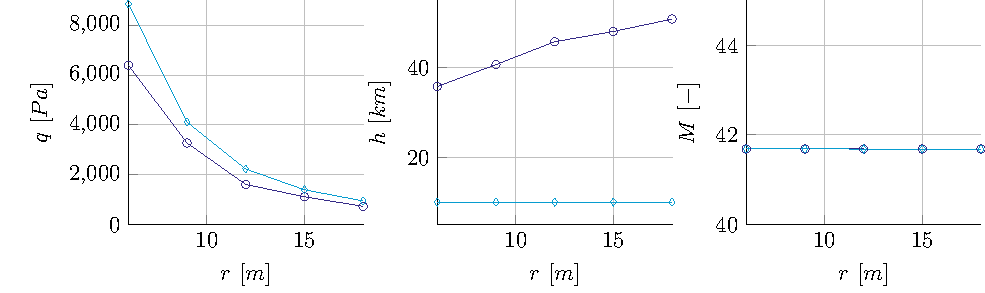
\includegraphics[width=\textwidth]{./Figure/orbit/radius_param.pdf}
	\caption{maximal dynamic pressure, height and Mach number for different radii}
	\label{fig:radius}
\end{figure}


Apart from this results it should be noted that there is a lower limit to the diameter of the aeroshell imposed by the side heatflux into the capsule. For a large diameter the capsule is in the wake of the aeroshell and the side heatflux can thus be negelcted. For a smaller diameter aeroshell eventually a backshell will be needed to protect the capsule. This will induce a inacceptable amount of weight.

\paragraph{Entry corridor}

The entry corridor is the fictional box where the re-entry vehicle should pass through to go into orbit. To low and the acceleration limit or the heat limit is breached, to high and the re-entry vehicle will skip on the atmosphere and never return. This corridor is dependent on different design parameters, the most important are the aerodynamic coefficients, entry velocity and control system.

\paragraph{Effect of initial flight path angle}

\begin{figure}[H]
	\centering
	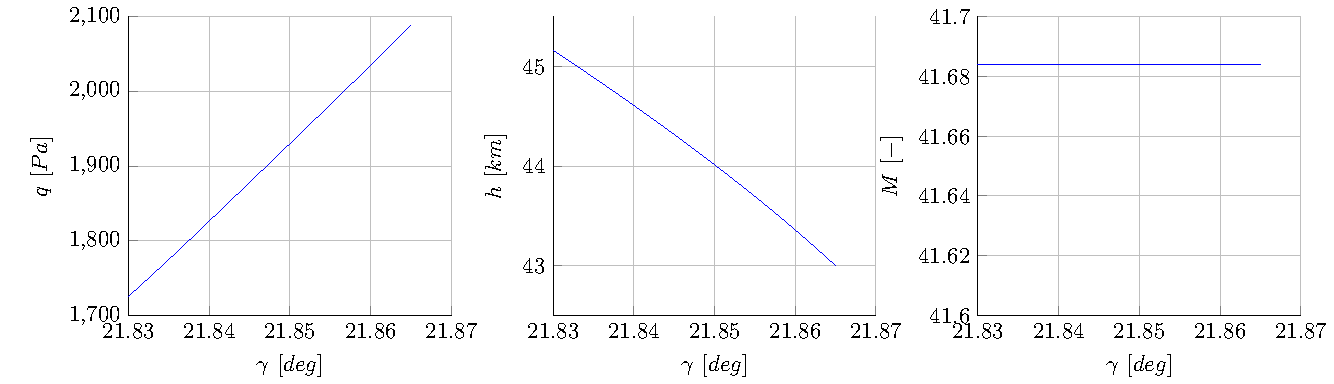
\includegraphics[width=\textwidth]{./Figure/orbit/effectgamma.pdf}
	\caption{Effect on dynamic pressure, height and Mach number for different flight path angles}
	\label{fig:effectgamma}
\end{figure}

\paragraph{Effect of angle of attack}

\begin{figure}[H]
	\centering
	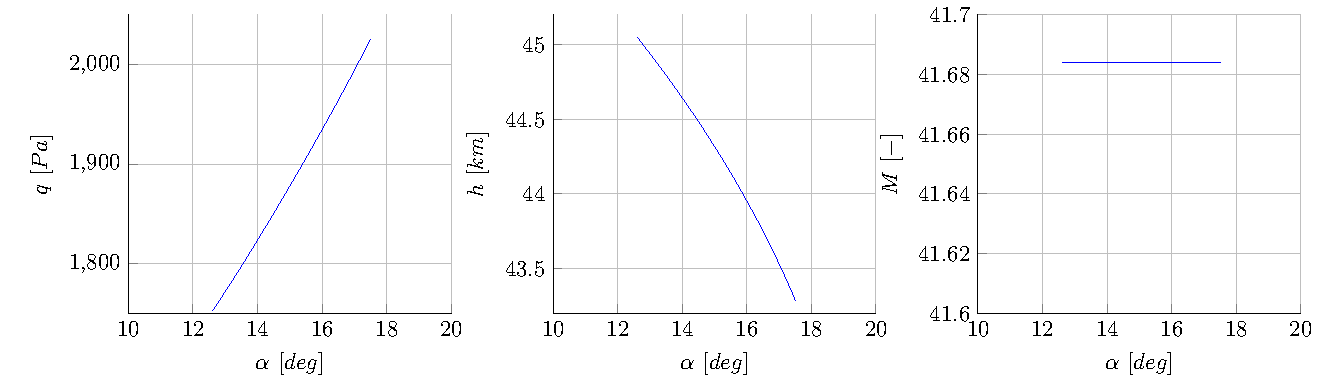
\includegraphics[width=\textwidth]{./Figure/orbit/effectalpha.pdf}
	\caption{Effect on dynamic pressure, height and Mach number for different angles of attack}
	\label{fig:effectalpha}
\end{figure}

\paragraph{Effect of bank angle}

\begin{figure}[H]
	\centering
	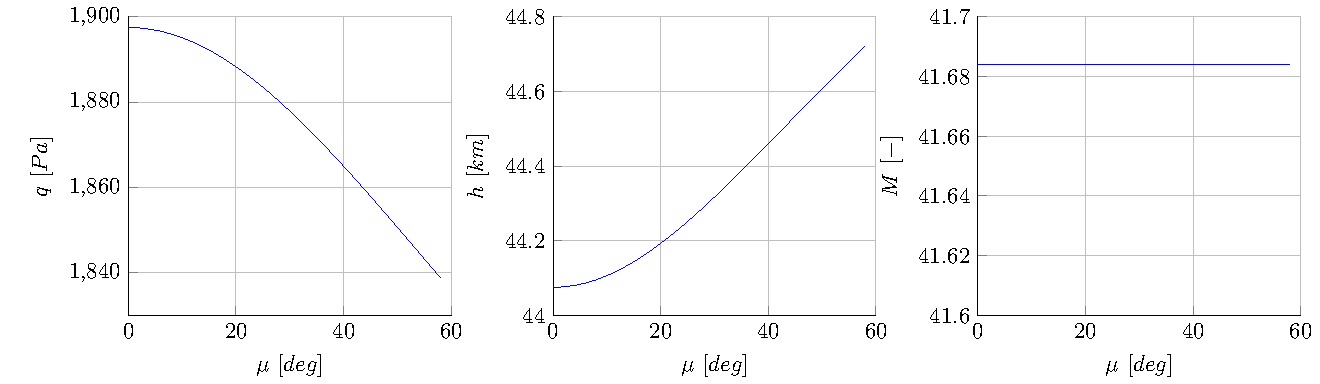
\includegraphics[width=\textwidth]{./Figure/orbit/effectmu.pdf}
	\caption{Effect on dynamic pressure, height and Mach number for different bank angles}
	\label{fig:effectmu}
\end{figure}


